\chapter{The \match* step}
\label{chap:matching}

The \match* step has the objective of leveraging the different camera views to estimate the depth (and, consequently, the 3D coordinates) of the bubbles.
The depth estimation is done with the technique of stereoscopy (see section~\ref{sec:backgr:stereo}).
In particular, the \match* step needs to match the same bubble across different cameras, to then call \texttt{OpenCV}'s \texttt{triangulatePoints} function for reconstructing the 3D position.

\section{Requirements}

\subsection{Input}

Depending on the pipeline order, the input to the \match* step can be either the output of the \locate* step or the one of the \linkDD* step.
In both cases, the input is composed of two arrays:
\begin{itemize}
	\itemsep 0em
	\item the array of the coordinates \texttt{positions[C][F][B]} (described in sections~\ref{sec:locate:output} and \ref{sec:linkDD:output}), which has the same format in both cases;
	\item the representation of valid coordinates, which varies based on the previous step: \locate* has a \texttt{numTracers[C][F]}, as explained in section~\ref{sec:locate:output}, while \linkDD* uses a larger \texttt{validTracers[C][F][B]}, described in section~\ref{sec:linkDD:output}.
\end{itemize}
In both cases, the \match* operates on the coordinates of the valid 2D coordinates: an initial step extracts such coordinates from the \texttt{positions} array, leveraging the other array in the correct way.
After that, the \match* can be executed without caring about the source of the data.

\subsection{Output}
\label{sec:match:output}

The \match* step's output consists in a couple of arrays, similar to the output of the \linkDD* (see section~\ref{sec:linkDD:output}).

The 3D coordinates of the bubbles are stored in a three-dimensional, floating array called \texttt{positions}. \texttt{positions[F][B]} contains the coordinate of the $B$-th bubble in the $F$-th time instant, as a tuple \texttt{(x, y, z)}.
The camera index disappeared, since this step combines the information from all cameras into a single, 3D description of the bubbles.

To represent the valid bubbles, a three-dimensional, boolean \texttt{validTracers} array is used.
\texttt{validTracers[F][B]} marks whether \texttt{positions[F][B]} contains a valid position or not.
Similarly to the \texttt{positions} array, the passage from 2D to 3D removes the dimension of the camera index.

Depending on the source of data, this step can either produce plain 3D coordinates, or 3D tracklets.
If the input is the \locate* step, then the bubble coordinates will be all grouped towards smaller $B$s, and there will be no correlation between bubbles with the same index in consecutive frames.
Instead, if the input is the \linkDD* step, the distribution of real coordinates within the $B$ dimension of the arrays will be less regular, due to the added constraint that ``same value for $B$ implies same real bubble''.

\subsection{Speed}

To respect the real time constraint, the \match* step should operate at 30 FPS, ideally independently of the number of cameras.

\subsection{Quality}

The matching algorithms start from a bubble in one camera, and try to find the matching bubble on the other cameras.
Such attempt can have three outcomes:
\begin{itemize}
	\itemsep 0em
	\item correct match: the bubble is matched to the correct one in the other camera. This is the ideal case, since it would lead to a correct 3D reconstrucion;
	\item missing match: the original bubble is not matched to another one. Since the setup is composed by more than 2 cameras, a missed match is not too terrible, since it is still possible that the matches in the other cameras are correct, to have a correct 3D reconstruction;
	\item wrong match: the bubble is matched to a wrong one. This leads to certain reconstrucion errors, since the \texttt{triangulatePoints} function will have either wrong or incoherent information.
\end{itemize}
The ideal matching algorithm is therefore one that produces correct matches for all bubbles, but if it's not possible, it's better to have missing matches rather than wrong matches.

\section{State of the art}

For the \match*, no existing solution was found when looking on the Internet: the matching is usually done on full images, not on single sets of cordinates.
The only starting point available for this step was the original tool developed by the research group, the objective of the acceleration.
In particular, it allows to choose between an epiline-only approach (examined in section~\ref{sec:match:epiline}) and a brute force algorithm (evaluated in section~\ref{sec:match:bruteforce}).

\section{Approaches}

The following chapters describe the different approaches explored for the \match* step
The evaluation was performed separately for speed and quality, with the speed measured on the same dataset as the \linkDD* step.
For the quality, it was not possible to have a ground truth containing the correct match between two cameras, neither with a real dataset nor with a synthetic one.
As such, a manual classification of correct/missed/wrong matches was done.
As visible in figure~\ref{fig:match:example}, the displacement between the view of two cameras is mostly constant: checking this consistency allows a human eye to evaluate the correcness of a match.

The qualitative evaluation was performed using two Blender-generated datasets, composed by a single frame, with respectively 30 and 100 bubbles.
An attempt was done with more bubbles, but the image was too crowded to identify correct or wrong matches.

\begin{figure}[H]
	\centerline{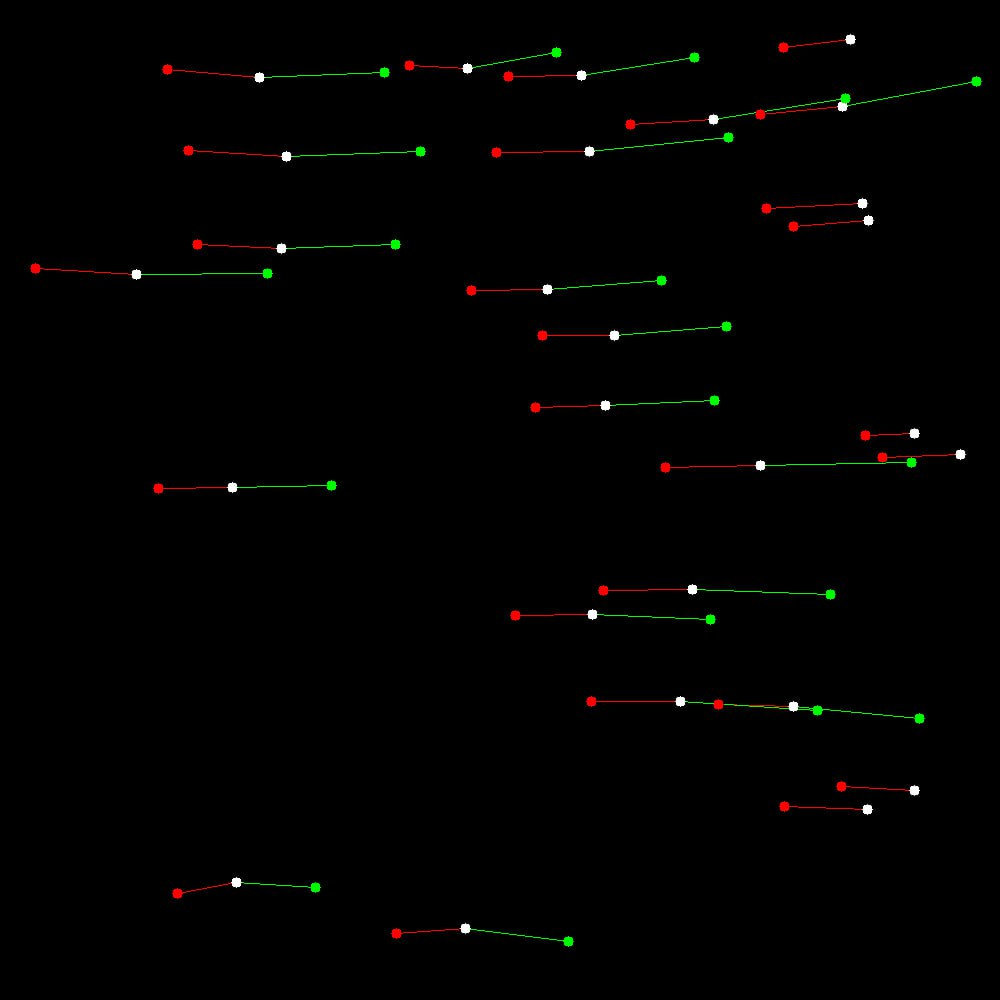
\includegraphics[width=0.8\textwidth]{images/match-observation.png}}
	\caption{\centering An example of \match*: the bubbles seen by the main (white) camera, matched to the corresponding bubbles seen from the other two (red, green) cameras}
	\label{fig:match:example}
\end{figure}

\newpage
\subsection{Long trajectory}
\label{sec:match:traj}

The research group that commissioned this thesis was working in parallel on a way to estimate calibration data without the need of a calibration process.
Instead, the model developed tried to perform a \match* (without knowledge of the epilines), to infer the calibration data from it.
Since this task was in common among the two projects, their solution was also considered and evaluated for the scope our purpose.

\subsubsection{Algorithm}

The solution uses a Deep Learning model, Lightglue~\cite{lightglue}, to match long trajectories seen from different cameras.
In particular, the model performed the match on a specific frame by looking at the 200-frames-long trajectories that started in the frame itself.

\subsubsection{Evaluation}

While this approach was useful in the complex situation of auto-calibration, for our task it was too computationally intensive.
Indeed, the maximum speed obtainable with this approach was 3 FPS, too far from the target 30 FPS.
 \newpage
\subsection{Closest to epiline}
\label{sec:match:epiline}

\subsubsection{Algorithm}

\subsubsection{Evaluation}
 \newpage
\subsection{Epilines + median correction}
\label{sec:match:epi-median}

As previously stated, the offset between two camera views of the same bubble is consistent across all the bubbles in the scene.
This fact is used in this approach to find and potentially correct mistakes.
Originally, the average displacement was hypothesized to be a good comparison term for detecting errors, but it would be very sensitive to errors.
Instead, the median displacement is used, since the number of errors in one direction is estimated to cancel out the number of errors in the opposite direction: this leaves the correct displacements towards the center range.
The median used is a vector whose components are the medians of the displacement components.
As an example, displacements of $(10, 1)$, $(11, 0)$ and $(-3, -1)$ would generate a median displacement of $(10, 0) = \left( med(10, 11, -3), med(1, 0, -1) \right)$.


\subsubsection{Algorithm}

For non-main camera is processed with the following steps:
\begin{enumerate}
	\itemsep 0em
	\item For each bubble in the main frame:
	      \begin{enumerate}
		      \item Compute the coefficients $a$, $b$ and $c$ of the epiline $ax+by+c{=}0$;
		      \item Compute the distance (with a scale factor) of all bubbles $(x_i, y_i)$ in the side camera from the epiline: $d_i = ax_i + by_i + c$;
		      \item Select as candidate match the bubble with $d=min_i(d_i)$;
		      \item Compare $d$ with the reasonability threshold $T$:
		            \begin{itemize}
			            \item If $d<T$, consider the bubble as a valid (temporary) match;
			            \item Otherwise, consider the original bubble as unmatched.
		            \end{itemize}
	      \end{enumerate}
	\item Compute the median of all the matches of the frame;
	\item For each bubble in the main frame:
	      \begin{enumerate}
		      \item Compute the displacement and compare it with the median:
		            \begin{itemize}
			            \item If both the difference in length and the angle between the vectors are under specific thresholds, confirm the match, and continue with the next bubble;
			            \item Otherwise, correct the match by performing the following steps;
		            \end{itemize}
		      \item With a procedure similar to steps 1.a to 1.d, find the $N$ (parameter) bubbles closest to the epiline;
		      \item Among them, find the one whose displacement is the most similar to the median displacement;
		      \item Check the correctness of this new match:
		            \begin{itemize}
			            \item If the bubble is further than the threshold $T$ (step 1.d) from the epiline, consider the match wrong and remove it;
			            \item If the new displacement still does not satisfy the distance and angle from the median, consider the match wrong and remove it;
			            \item Otherwise, correct the previous match with this one.
		            \end{itemize}
	      \end{enumerate}
\end{enumerate}

\subsubsection{Evaluation}

Clearly, the introduction of the epilines check slowed down the algorithm, that can now process 55 frames per second.
However, the speed was traded with an improvement on the quality: for the 30-bubbles dataset, the distribution of correct/missed/wrong matches was 27/2/1, and 74/20/6 for the 100-bubbles dataset.
 \newpage
\subsection{Epilines + short trajectory}
\label{sec:match:epi-traj}

\subsubsection{Algorithm}

\subsubsection{Evaluation}
 \newpage
\subsection{Epilines + KNN}
\label{sec:match:epi-knn}

Traditional stereoscopy finds the correct pixel on the epiline by comparing the patch around the original pixels to patches around the epiline.
This idea of ``looking at the neighborhood'' was evolved to our case into a k-Nearest Neighbor search.

\subsubsection{Algorithm}

The algorithm processes each camera with the following steps:
\begin{enumerate}
	\itemsep 0em
	\item Compute the kNN of all bubbles of both the main and the side cameras, storing them as relative offsets from the bubble's position;
	\item For each bubble in the main camera:
	      \begin{enumerate}
		      \item Compute the coefficients $a$, $b$ and $c$ of the epiline $ax+by+c{=}0$;
		      \item Compute the distance (with a scale factor) of all bubbles $(x_i, y_i)$ in the side camera from the epiline: $d_i = ax_i + by_i + c$;
		      \item Consider only the bubbles with $d_i<T$, for a specific threshold $T$ (if there are none, leave the bubble unmatched);
		      \item Compute the cosine similarity between the bubble in the main camera and the others, considering the positions of the kNNs;
		      \item Select as match the bubble with highest cosine similarity, provided that it has at least a minimum value for that (if not, leave the bubble unmatched).
	      \end{enumerate}
\end{enumerate}

\subsubsection{Evaluation}

Similarly to the previous approach, this algorithm has an acceptable speed (122 FPS), but an extremely bad quality, with 2/28/0 correct/missed/wrong matches in the 30-bubbles dataset, and 1/98/1 in the 100-bubbles dataset.
 \newpage
\subsection{Brute force}
\label{sec:match:bruteforce}

This approach is one of the two implemented in the original MATLAB script: it leverages the fact that more than two cameras are present, not only as a confirmation, but as a knowledge-extracting method.

Given a bubble on the main camera, it should be matched to a specific bubble on the other two cameras.
If the 3D position is reconstructed from the main and one side camera, the result should be similar to the reconstruction done with the main and the other side camera.
On the other side, wrong matches would reconstruct totally different 3D coordinates.

\subsubsection{Algorithm}

\begin{enumerate}
	\itemsep 0em
	\item For each bubble in the main camera:
	      \begin{enumerate}
		      \item Reconstruct the 3D position, matching it with all the bubbles on one non-main camera. The result will be a set of 3D points ($P_i$);
		      \item Do the same, with the other non-main camera (to obtain a set $P_j'$);
		      \item Find the points $p\in P_i$ and $p'\in P_j'$ whose distance is the smallest;
		      \item Check their distance:
		            \begin{itemize}
			            \item If it is below a specific threshold, the two reconstructions are considered to be the same bubble, hence the two matches are approved;
			            \item Otherwise, the reconstructed bubbles are the closest plausible, but still different bubbles, hence the match is considered missing.
		            \end{itemize}
	      \end{enumerate}
\end{enumerate}

\subsubsection{Evaluation}

This approach was not evaluated directly, since just limiting to the bubbles close to the epiline could highly reduce its computational cost.
This algorithm was therefore only considered as starting idea for the approach described in the next paragraph.
 \newpage
\subsection{Epilines + brute force}
\label{sec:match:epi-bruteforce}

Given the knowledge that the correct match is near the epiline, there is no need to perform a brute force check on all the bubbles, as proposed in the previous approach.
Instead, it is enough to check the bubbles close to the epiline.

\subsubsection{Algorithm}

\begin{enumerate}
	\itemsep 0em
	\item For each bubble in the main camera:
	      \begin{enumerate}
		      \item Compute the distance $d$ (with a scale factor) of all bubbles in each side camera to the corresponding epiline;
		      \item Consider only the bubbles with $d<T$, for a specific threshold $T$ (if there are none, leave the bubble unmatched);
		      \item Reconstruct the 3D position matching it with all the bubbles on one side camera. The result will be a set of 3D points ($P_i$);
		      \item Do the same, with the other side camera (to obtain a set $P_j'$);
		      \item Find the points $p\in P_i$ and $p'\in P_j'$ that minimize their distance;
		      \item Check their distance:
		            \begin{itemize}
			            \item If it is below a specific threshold, the two bubbles are considered the same, and the two matches are approved;
			            \item Otherwhise, the reconstructed bubbles are the closest plausible, but still different bubbles, hence the match is considered missing.
		            \end{itemize}
	      \end{enumerate}
\end{enumerate}

\subsubsection{Evaluation}

This approach yields excellent result, with no mistakes recorded.
This is achieved thanks to its requirement to have a ``3-way confirmation'' on the bubbles: when in doubt, it prefers to leave the bubble unmatched.
The qualitative result were 18/12/0 correct/missing/wrong matches on the 30-bubbles frame and 55/45/0 on the 100-bubbles dataset.
This however comes at a slight cost of speed, since this algorithm is only able to reach 19 FPS.
 \newpage

\section{Final choice}

Figure~\ref{fig:match:comparison} compares speed and quality of the different approaches.
Due to the real-time constraint, the long trajectories and the brute force algorithms are discarded.
Among the remaining approaches, the median approach is the best one, hence it is the selected one. 

\begin{figure}
	\centerline{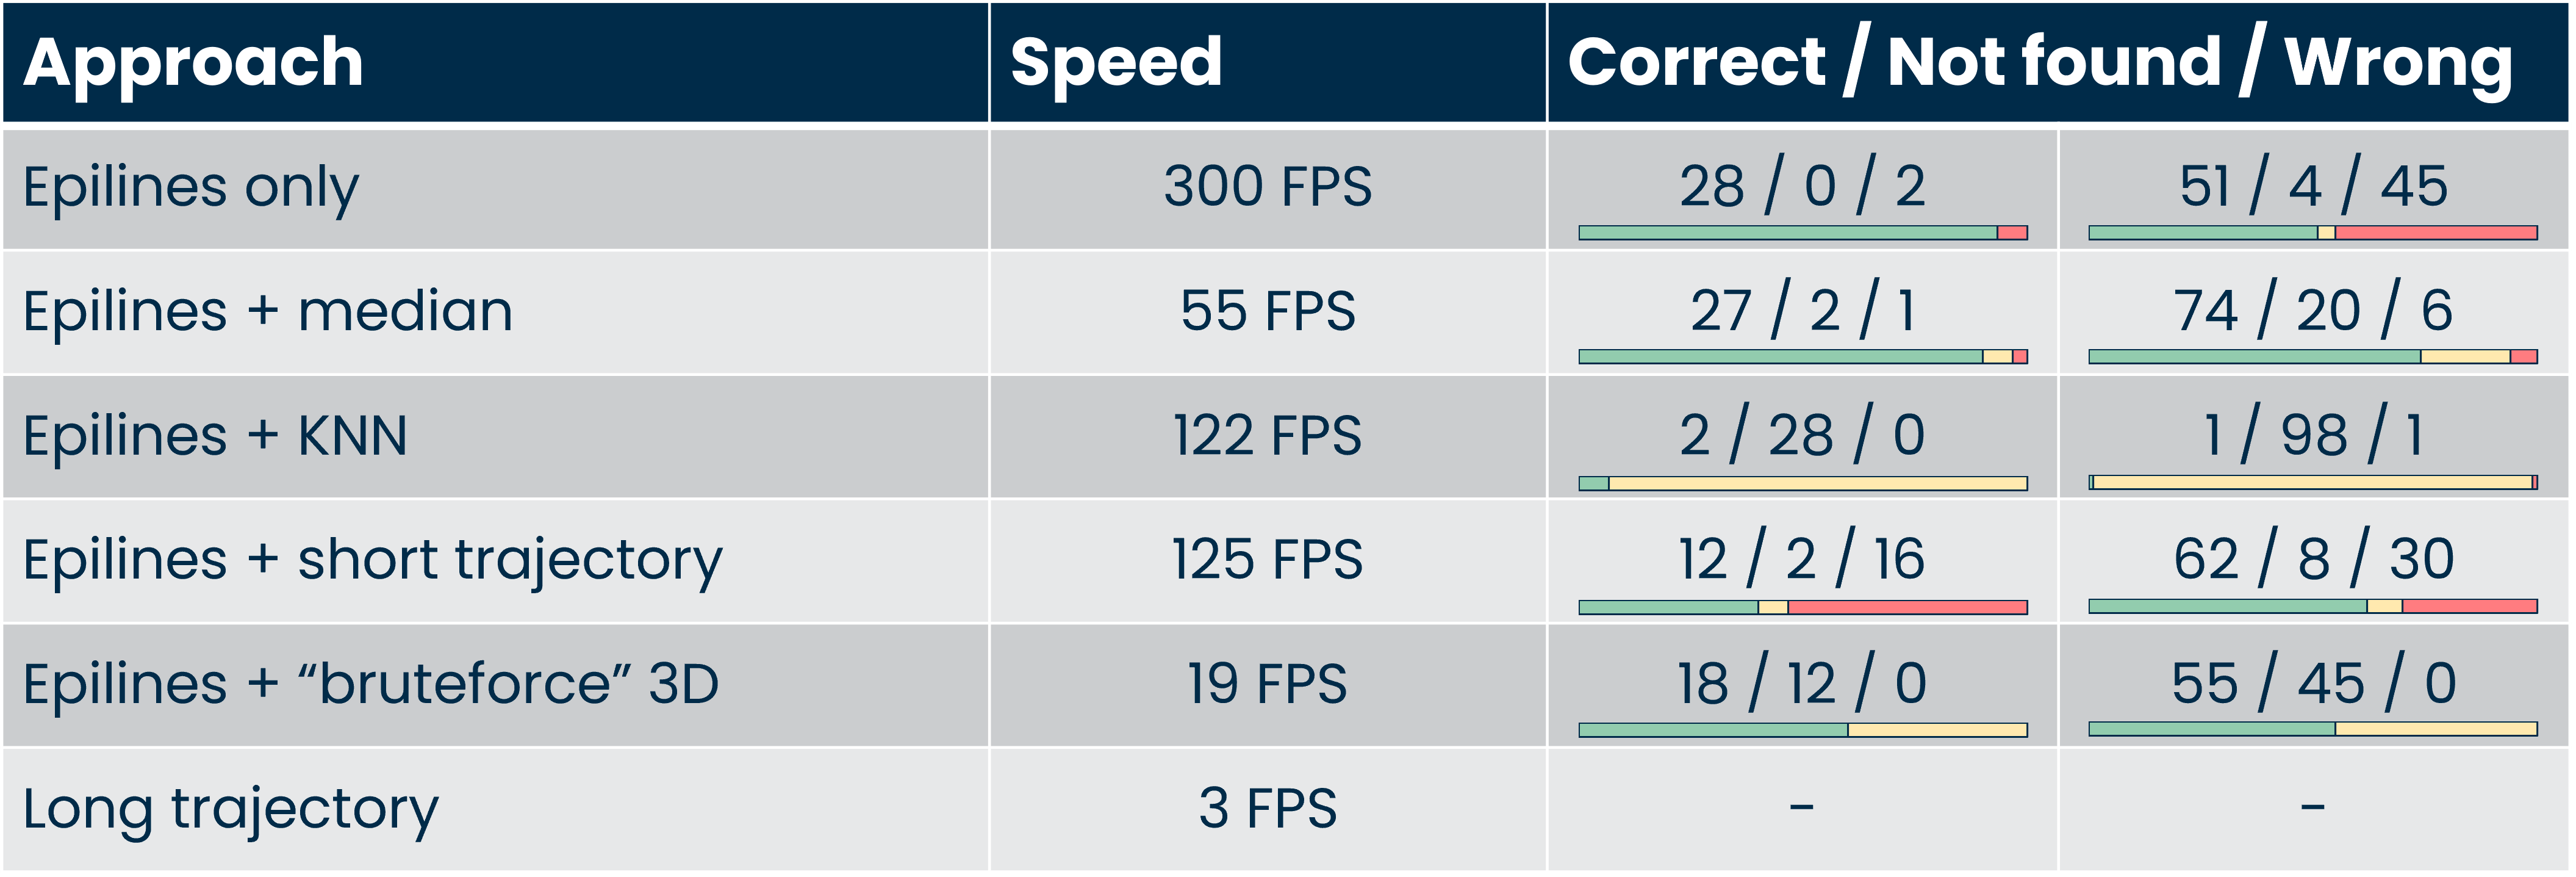
\includegraphics[width=0.9\textwidth]{images/3d-matching-comparison-without-chosen.png}}
	\caption{\centering Comparing speed and quality of the various \match* approaches}
	\label{fig:match:comparison}
\end{figure}
